\section{Auswertung}

\subsection{Strahlungsbelastung}

Da für das Experiment radioaktive Präparate benutzt werden, scheint eine
Abschätzung der maximalen, persönlichen Belastung sinnvoll.

Folgende Annahmen wurden getroffen:
\begin{itemize}
  \item Die betreffende Person wiegt $m = \SI{80}{\kilo\gram}$.
  \item Die Einwirkdauer beträgt jeweils $s = \SI{12}{\hour}$.
  \item Die Aktivität $A$ aller 3 Präparate übersteigt jeweils nicht
        \SI{4e5}{\becquerel}.
  \item Die Halbzeit $t$ aller 3 Präparate wird mit dem maximalen Wert, 30 Jahren,
        abgeschätzt.
  \item Seit der Vermessung der Präparate sind aufgerundet $u = $ 3 Jahre vergangen.
  \item \SI{100}{\percent} der Strahlung wird aufgenommen.
  \item Der Strahlungsgewichtungsfaktor für γ-Strahlung beträgt 1.
  \item Die γ-Quanten haben eine maximale Energie von
        $E = \SI{0.7}{\mega\eV} = \SI{1.12e-13}{\joule}$
  \item Es gibt $n = 3$ Proben.
\end{itemize}
Damit berechnet sich die radioaktive Belastung zu
\begin{equation}
  s \left(\frac{1}{2}\right)^{u/t} n E A / m = \SI{0.07}{\milli\sievert}
\end{equation}
und macht somit bei einer durchschnittlichen Strahlungsbelastung in Deutschland von
\SI{4.3}{\milli\sievert} pro Jahr rund \SI{2}{\percent} aus.

\subsection{Signalbetrachtung}
TODO

\subsection{Latenzzeit der Messtechnik}

\begin{figure}[htb]
      \centering
      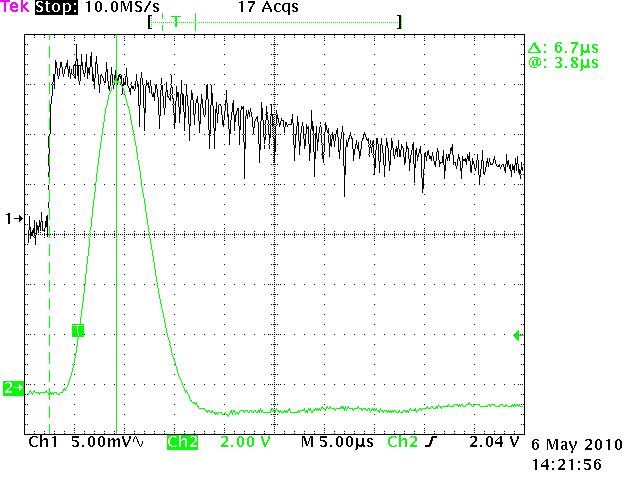
\includegraphics[width=1\columnwidth,keepaspectratio]{messverzoegerung}
      \caption{Standbild des Digital-Oszilloskops zur Messung der Latenzzeit}
      \label{fig:latenz}
\end{figure}

Durch die Verwendung des Hauptverstärkers kann das Signal mit höherer Präzision
gemessen werden, jedoch muss man dafür eine zeitliche Verzögerung $Δt$ in Kauf
nehmen. Um jene zu bestimmen, wird der Trigger des Oszilloskops auf den
Vorverstärker gestellt und das Bild manuell im richtigen Moment angehalten, so
dass im Ergebnis ein Standbild wie in \fref{latenz} exportiert werden kann.
\begin{table}[htbp]
\centering
% \setlength{\tabcolsep}{14pt}
\begin{tabular*}{\columnwidth}{%
S[tabformat=1.1]%
S[tabformat=1.1]%
S[tabformat=1.1]%
S[tabformat=1.1]%
S[tabformat=1.1]%
S[tabformat=1.1]%
S[tabformat=1.1]%
S[tabformat=1.1]%
}
\toprule
{$x_1$} & {$x_2$} & {$x_3$} & {$x_4$} & {$x_5$} & {$x_6$} & {$\bar x$} & {$Δx$}\\
\midrule
6.7 & 6,8 & 6,5 & 6.8 & 6.8 & 6.6 & 6.7 & 0.1 \\
\bottomrule
\end{tabular*}
\label{tab:latenzmesswerte}
\caption{Messwerte der Latenzzeit}
\end{table}
Die Messergebnisse sind in \tref{latenzmesswerte} enthalten. Wenn man den Fehler
der einzelnen Messung mit \num{0,1} als letzte signifikante Stelle abschätzt, so
kann der Fehler des Mittelwerts auch insgesamt großzügig mit \num{0.1} abgeschätzt
werden. Die Latenzzeit beträgt somit
\begin{equation}
  Δt = \SI{6.7(1)}{\second}
\end{equation}
. Da die Öffnungszeit jedoch vom Computer vollautomatisch gemessen wird, ist
eine Latenzzeit in diesen Versuch unerheblich.

\subsection{Untergrundmessung}

\subsection{Eichung}


